\documentclass[a5paper]{article}
\usepackage{graphicx}
\usepackage{hyperref}
\usepackage[final]{pdfpages}
\usepackage[parfill]{parskip}% don't indent new sections
\usepackage[utf8]{inputenc}
\usepackage{listings}
\usepackage{color}
\usepackage[a4paper]{geometry}
\pagestyle{empty}

\definecolor{dkgreen}{rgb}{0,0.6,0}
\definecolor{gray}{rgb}{0.5,0.5,0.5}
\definecolor{mauve}{rgb}{0.58,0,0.82}

\lstset{frame=tb,
    language=Java,
    aboveskip=3mm,
    belowskip=3mm,
    showstringspaces=false,
    columns=flexible,
    basicstyle={\small\ttfamily},
    numbers=left,
    numberstyle=\tiny\color{gray},
    keywordstyle=\color{blue},
    commentstyle=\color{dkgreen},
    stringstyle=\color{mauve},
    breaklines=true,
    breakatwhitespace=true,
    tabsize=3
}

\title{Practical Concurrent and Parallel Programming}
\author{Emil Lynegaard}

\begin{document}

\includepdf[pages=1]{res/front_page.pdf}

\newpage
\tableofcontents
\newpage

\maketitle
\textit{I hereby declare that I have answered thede exam questions myself without any outside help.}\\

Thoughout the report, I will be using inline code snippets, but include full files in the appendix. For all tests, the same machine will be used. Table \ref{table:sysinfo} contains the results of \texttt{SystemInfo}:

\par\noindent\rule{\textwidth}{0.4pt}
\begin{table}[!ht]
\begin{center}
\begin{tabular}{ l l }
OS & Linux; 4.13.12-1-ARCH; amd64\\
JVM & Oracle Corporation; 1.8.0\_144\\
CPU & null; 8 "cores"\\
Date & 2017-12-11T09:20:13+0100
\end{tabular}
\end{center}
\caption{System Info}
\label{table:sysinfo}
\end{table}
\par\noindent\rule{\textwidth}{0.4pt}
\newpage

\section{Question 1}
\subsection{}
Seeing as we are interested in seeing how well each implementation performs on random input of different sizes, we use Mark9 for the benchmarking, as it calculates the per element mean time and standard deviation.

\begin{figure}[!ht]
    \centering
    \noindent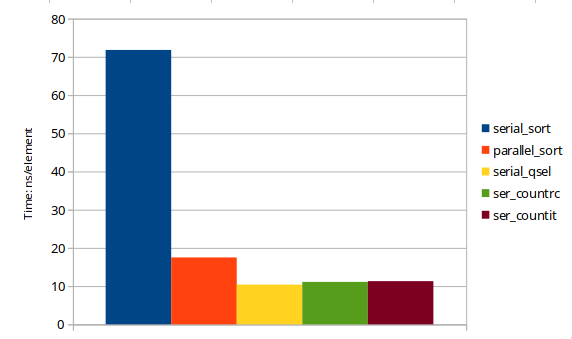
\includegraphics[scale=0.5]{res/graph_q1.png}
    \caption{Plot of running times of given implementations. Tested with input size $10^7$.}
    \label{fig:graphq1}
\end{figure}

From Graph \ref{fig:graphq1} we see that, perhaps unsurprisingly, the serial \texttt{quickSelect} and \texttt{quickCount} implementations beat out serial sort entirely.
We do however see parallel sort get rather close to the expected linear running time implementations, due to the test machine having a quad-core CPU,
allowing an approximate 4 time speedup from the serial implementation. Between the expected linear running time algorithms, serial \texttt{quickSelect} beats out its \texttt{quickCount} counterparts. This may be due to \texttt{quickSelect} avoiding spending time allocating new memory, other than its initial copy.

\subsection{}
Below is shown a parallel \texttt{quickCount} implementation using tasks, where \texttt{quickCountItTask} is the main function, and \texttt{filter} is the auxiliary method
in which the parallel filtering is done. The filter method mainly serves to reduce code duplication as the original implementation is near identical
for the filtering cases where we either have a too larger or a too small selected partition number.

To allow multiple tasks to safely increment \texttt{count}, we use a \texttt{final AtomicInteger} on line 28. In general for each iteration, all variables that we need to access
from within the threads are made final, as we get compile errors otherwise. For task partitioning, we try to split up the input array in even intervals skipping the partition element. For undivisible numbers,
we give the leftovers to the last created task. This can slow us down a little bit, since one task may end up doing more work than the others. In \texttt{filter} we take the same
approach to partitioning, and now use an \texttt{AtomicInteger} on line 8, to safely keep track of what index in the new array \texttt{m} we want to insert the next value in. This ensures that
we never try to write to the same index of \texttt{m} twice.

Other than these parallization measures, the overall structure of \texttt{quickCountItTask} is similar to that of the given \texttt{quickCountTask}.

\begin{lstlisting}
// Takes an arr, a partition, the size of the output array and a BiFunction,
// returning an array of the given size containing elements from arr for which 
// f.apply(arr[i], partition) returns true.
public static int[] filter(int[] arr, int partition, int size,  BiFunction<Integer,Integer,Boolean> f){
    int[] m = new int[size];
    ArrayList<Callable<Void>> filterers = new ArrayList<>();
    final AtomicInteger j = new AtomicInteger(0);
    final int step = arr.length/threadCount;
    for(int i=0;i<threadCount;i++) {
        final int from = i==0 ? 1 : i*step;
        final int to = i==threadCount-1 ? arr.length : i*step+step;
        filterers.add(() -> {
            for(int h= from; h<to; h++)
                if(f.apply(arr[h],partition)) m[j.getAndIncrement()]=arr[h];
            return null;
        });
    }
    try{ executor.invokeAll(filterers);
    } catch (InterruptedException e) { System.err.println("Threads interrupted");}
    return m;
}

static ExecutorService executor = Executors.newWorkStealingPool();
public static int quickCountItTask(int[] in) {
    int target = in.length/2;
    do {
        final AtomicInteger count = new AtomicInteger(0);
        final int[] inp = in;
        final int n = inp.length, p = inp[0];
        final int step = n/threadCount;

        //Counting
        ArrayList<Callable<Void>> counters = new ArrayList<>();
        for(int i=0;i<threadCount;i++) {
            final int from = i==0 ? 1 : i*step; //skip pivot
            //for undivisible numbers, just let the last thread take a larger chunk
            final int to = i==threadCount-1 ? inp.length : i*step+step;
            counters.add(() -> {
                for(int j = from; j<to; j++)
                    if(inp[j]<p) count.getAndIncrement(); 
                return null;
            });
        }
        try{ executor.invokeAll(counters);
        } catch (InterruptedException e) { System.err.println("Threads interrupted");}

        if (count.get() == target) return p; //Terminated

        //Filtering
        boolean tooLargeP = count.get() > target;
        int size = tooLargeP ? count.get() : n-count.get()-1;
        if(tooLargeP) {
            in = filter(inp, p, size, (x,y) -> x < y);
        } else {
            in = filter(inp, p, size, (x,y) -> x >= y);
            target=target-count.get()-1;
        }
    } while( true );
}
\end{lstlisting}
\subsection{}
Since the machine used for testing has 4 physical cores, this is the ideal amount of threads for the quickSelectIt. There is however only little difference between 4 and 8 since it supports hyperthreading\footnote{https://ark.intel.com/products/80806/Intel-Core-i7-4790-Processor-8M-Cache-up-to-4\_00-GHz}. Because of this, I have set the \texttt{threadCount} to 4, and tested with various input sizes. Figure \ref{fig:compTask} depicts the results. 
\begin{figure}[!ht]
    \centering
    \noindent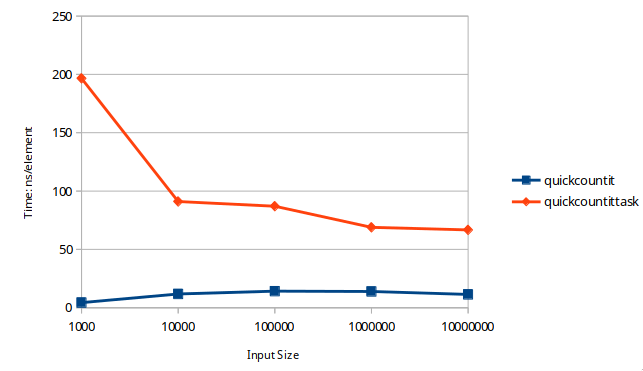
\includegraphics[scale=0.5]{res/graph_task.png}
    \caption{Plot of running times per element between \texttt{quickCountIt} and \texttt{quickCountItTask}}
    \label{fig:compTask}
\end{figure}

Perhaps in contrast to the expected outcome, \texttt{quickCountItTask} remains slower than \texttt{quickCountIt} even for large inputs. This can be due to how much it slows down on small inputs, with near $200ns/element$ for inputs of size $10^3$. Based on the Figure \ref{fig:compTask} it seems that it will not be able to catch up to the serial implementation no matter the input size.

\subsection{}
We assume that a single partioning step indicates one entire iteration of the \texttt{do-block} including counting and filtering. To test a single partioning step we temporarily modify \texttt{quickCountItTask} to return after a single iteration. Table \ref{table:constn} depicts the running time per element for inputs of size $10^4$ with a varying number of threads for a single step. Here we see that on smaller input sizes, the overhead of using multiple threads becomes increasingly noticable.

\begin{table}[ht!]
\centering
\begin{tabular}{|l|l|l|l|l|l|l|}
\hline
Threads          & 1    & 2    & 4    & 8    & 16   & 32   \\ \hline
Time: ns/element & 15.0 & 28.4 & 32.7 & 35.7 & 35.9 & 36.4 \\ \hline
\end{tabular}
\caption{Running times per element for a single partitioning step in \texttt{quickCointItTask}, with input size $10^4$, and a varying thread count}
\label{table:constn}
\end{table}

Similarly we also try to pin the thread count to 4 and vary the input size. This is depicted in Table \ref{table:constt}. Here we see that with the pinned thread count, we seem to scale positively in the size of the input up until $10^6$. This makes sense in terms of the benefits of multithreading outweighing the overhead, when each thread gets a sufficiently large part of the input to work with.

\begin{table}[ht!]
\centering
\begin{tabular}{|l|l|l|l|l|l|l|}
\hline
Input size       & $10^3$ & $10^4$ & $10^5$ & $10^6$ & $10^7$ & $10^8$ \\ \hline
Time: ns/element & 26.7 & 32.5  & 32.4   & 18.1    & 19.7     & 22.4      \\ \hline
\end{tabular}
\caption{Running times per element for a single partitioning step in \texttt{quickCointItTask}, with input size of thread count of 4 and varying input size}
\label{table:constt}
\end{table}

\subsection{}
To make our implementation a hybrid, we declare a constant \texttt{CUTOFF} and add the following line to the top of the \texttt{do-block} in \texttt{quickCountItTask}.
\begin{lstlisting}
if (in.length <= CUTOFF) return quickCountIt(in);
\end{lstlisting}

This change does make \texttt{quickCountItTask} faster, but even as a hybrid, it is unable to beat the sequential version, meaning that it still remains best to use the sequential version. This finding may either be due to the overhead of thread synchronization, or that the parallelization could be implemented in a more thread-friendly way.

\section{Question 2}
\subsection{}
\begin{lstlisting}
      (int) Arrays.stream(inp).skip(1).filter(i -> i < p).count();
\end{lstlisting}
Where \texttt{inp} is our input array, and \texttt{p} is our current partition candidate.
Skip the first element as this is the index of the partition element with which we do not wish to compare.

\subsection{}
\begin{lstlisting}
          Arrays.stream(inp).skip(1).filter(i -> i < p).toArray();
          Arrays.stream(inp).skip(1).filter(i -> i >= p).toArray();
\end{lstlisting}

\subsection{}
\begin{lstlisting}
public static int quickCountStream(int[] inp) {
    int partition=-1, count=0, n=inp.length;
    int target = n/2;
    do {
        partition=inp[0];
        final int p = partition;
        n=inp.length;
        count = (int) Arrays.stream(inp).skip(1).filter(i -> i < p).count();
        if (count == target) break;
        if (count > target){
            inp = Arrays.stream(inp).skip(1).filter(i -> i < p).toArray();
        }else{
            inp = Arrays.stream(inp).skip(1).filter(i -> i >= p).toArray();
            target=target-count-1;
        }
    } while( true );
    return partition; // we are on target
}
\end{lstlisting}

Combining the two we get above implementation, which yields correct results.

\subsection{}
\begin{lstlisting}
    Arrays.stream(inp).parallel().skip(1).filter(i -> i < p).count();
    Arrays.stream(inp).parallel().skip(1).filter(i -> i < p).toArray();
    Arrays.stream(inp).parallel().skip(1).filter(i -> i >= p).toArray();
\end{lstlisting}
Here we simply throw \texttt{.parallel()} onto the pipelines from before.

\subsection{}

\begin{lstlisting}
public static int quickCountStream(int[] inp) {
    int partition=-1;
    int target = inp.length/2;
    // Since we have to be working with boxed Integers. We start off by converting.
    List<Integer> list = Arrays.stream(inp).boxed().collect(Collectors.toList());
    do {
        partition = list.get(0);
        final Integer p = partition;
        Map<Boolean, List<Integer>> res = list.stream().skip(1).parallel()
            .collect(Collectors.partitioningBy(i -> i < p));

        List<Integer> smaller = res.get(true);
        List<Integer> bigger = res.get(false);

        if (smaller.size() == target) break;
        if (smaller.size() > target) list = smaller;
        else {
            target=target-smaller.size()-1;
            list = bigger;
        }
   } while( true );
    return partition; // we are on target
}
\end{lstlisting}
To avoid having to constantly do boxing, since Collectors does not work with primitives,
we start off by converting our \texttt([] inp) to \texttt{List<Integer>}.

The \texttt{partitioningBy} collector gives us a map of all with two entries.
The \texttt{true} entry on line 12, holding all elements larger than our partition element, and false entry on line 13 holding
all the elements larger than or equal to our partition element. The size of \texttt{smaller} now represents our \texttt{count}
from before, and the remainder of the code is similar to the given code.

\subsection{} 
In Figure \ref{fig:graphq2} we have tested all implementations from Figure \ref{fig:graphq1} again, and added the hybrid implementation as well as the stream implementations. Here the \texttt{CUTOFF} for the parallel iterative \texttt{quickCount} is set to $10^4$. Based on these tests, it appears that every parallel implementation is slower than the serial \texttt{quickSelect} and the serial recursive and iterative \texttt{quickCount}. While this is perhaps somewhat surprising, we can deduce that we either need smarter ways of parallelizing the implementations, or that \texttt{quickCount} does not lend itself positively to parallelization on my machine, despite it being very reasonable to implement.
\begin{figure}[ht!]
    \centering
    \noindent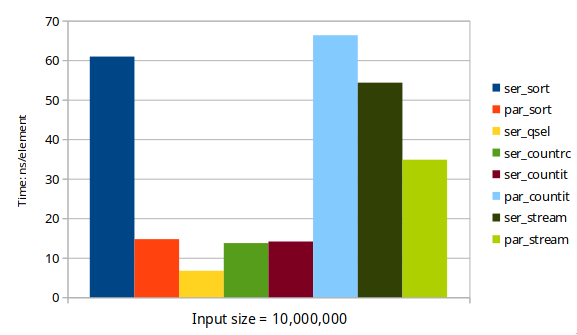
\includegraphics[scale=0.45]{res/graph_q2.png}
    \caption{Plot of running times including parallel iterative and stream based. Tested with input size $10^7$.}
    \label{fig:graphq2}
\end{figure}

\section{Question 3}
\subsection{CPU pinning:} If we assume that the total number of threads is equal to the number of cores on the machine of execution, CPU pinning can be advantageous if the program gets all of the machine's CPU time, and the list is evenly partitioned between threads. In these specific conditions, not having to schedule threads may be beneficial as these conditions should cause various threads to finish their iteration's work simultaneously. On the other hand, if the input is not evenly distributed and the system is using resources on other tasks as well, one partition may end up being poorly scheduled on a core with less free CPU time than one of the other available cores. Another benefit of thread pinning, which may be more significant, is that this will allow the threads to keep most of the relevant values in their designated cores' L1 cache, leading to less cache misses\footnote{https://en.wikipedia.org/wiki/CPU\_cache\#Cache\_miss}. This benefit may even extend to L2 cache for some CPUs\footnote{https://en.wikipedia.org/wiki/CPU\_cache#Cache\_hierarchy\_in\_a\_modern\_processor}.
\subsection{Load balancing:}
By having each thread own certain data ranges, we may end up with several threads having nothing or very little to do after few iterations. For example, if the input is near sorted and we assign threads consecutive ranges, some threads may up filtering out all their elements in the first iteration depending on the selected pivot.

\section{Question 4}
\subsection{}
Since \texttt{x} and \texttt{y} are parameters, we are not guaranteed to always grab locks in the same order, hence we are prone to dead-locks.

\subsection{}

\begin{lstlisting}
union(0,1)
union(1,0)
\end{lstlisting}

Above example when executed in parallel may lead to the first call grabbing the lock on \texttt{nodes[0]}, the second call grabbing the lock on \texttt{nodes[1]} and both calls thereafter waiting to get the lock on the node that their counterpart already grabbed.

\subsection{}
We modify the given \texttt{concurrent()} method in class \texttt{UnionFindTest} in file \texttt{MyUnionFind.java} to target the issue we identified in 4.1.
\begin{lstlisting}
public void deadlock(final int size, final UnionFind uf) throws Exception {
    final int[] numbers = new int[size];
    for (int i = 0; i < numbers.length; ++i) numbers[i] = i;
    final int threadCount = 32;
    final CyclicBarrier startBarrier = new CyclicBarrier(threadCount+1), 
          stopBarrier = startBarrier;
    Collections.shuffle(Arrays.asList(numbers));
    for (int i = 0; i < threadCount; ++i) {
        final boolean reverse = i%2==0;
        Thread ti = new Thread(new Runnable() { public void run() {
            try { startBarrier.await(); } catch (Exception exn) { }
            if (reverse)
                for (int j=0; j<100; j++)
                    for (int i = 0; i < numbers.length - 1; ++i) 
                        uf.union(numbers[i], numbers[i + 1]);
            else 
                for (int j=0; j<100; j++)
                    for (int i = 0; i < numbers.length - 1; ++i) 
                        uf.union(numbers[i + 1], numbers[i]);
            try { stopBarrier.await(); } catch (Exception exn) { }
        }});
        ti.start();
    }
    startBarrier.await();
    stopBarrier.await();
    final int root = uf.find(0);
    for (int i : numbers) {
        assertEquals(uf.find(i), root);
    }
    System.out.println("No deadlocks");
}
\end{lstlisting}

As seen from line 10 to 20, half the threads will now be attempting to union nodes in reverse order of the other half.
From my tests, calling the above defined \texttt{deadlock} method with parameters shown below, deadlocked every time.

\begin{lstlisting}
UnionFindTest test = new UnionFindTest();
test.deadlock(itemCount, new BogusFineUnionFind(itemCount));
\end{lstlisting}

By merely adding a check to the given \texttt{union()} method in class \texttt{BogusFineUnionFind} to ensure we always lock the lowest entry of the \texttt{nodes} array first, the deadlock test
executes without deadlocking.

\section{Question 5}
\textbf{Specifications}:
\begin{enumerate}
\item pop returns an inserted item or the value null. It might block until another concurrent operation completes, but it will return without delay if no other operation is happening simultaneously. In particular, it will not block until another thread inserts some element.
\item for each element that is pushed, there is at most one pop operation that returns that element.
\item If there are no further concurrent operations, pop will succeed (i.e. return a non-null value) if so far there
have been more successful push than pop operations.
\item If processor A pushed two elements x and y in this order, and processor B pops both elements, then this
happens in reverse order. (There is no further constraint on ordering).
\end{enumerate}

\subsection{}\label{sec:mystacksimple}
\begin{lstlisting}
import java.util.LinkedList;
public class MyStack<T> {
    private Object lock;
    private LinkedList<T> stack;

    public MyStack(){
        lock = new Object();
        stack = new LinkedList<T>();
    }

    public void push(T obj) {
        synchronized(lock){
            stack.push(obj);
        }
    }

    public T pop() {
        synchronized(lock){
            return stack.peek() != null ? stack.pop() : null;
        }
    }
}
\end{lstlisting}

Above generic implementation utilizes that Java's \texttt{LinkedList} ships with \texttt{push} and \texttt{pop}.
Alternatively we could use the combination \texttt{addLast} and \texttt{removeLast} or \texttt{addFirst} and \texttt{removeFirst} of which the second pair by Java's documentation is equivalent to \texttt{push} and \texttt{pop}\footnote{https://docs.oracle.com/javase/7/docs/api/java/util/LinkedList.html}. 
In \texttt{pop}, given that the specification states that we should return null if the list is empty, we use \texttt{peek} to check if there is a first element, if there isn't return null, otherwise \texttt{pop}.
The locking could also be done implicitly on \texttt{this} by marking the methods as synchronized, but here we use an explicit global lock object as it seems more in line with specification number 1.

\subsection{}
Given the initially stated  specifications, below are added bullet points (letters) matching specifications, describing why the implementation from \ref{sec:mystacksimple} is sufficient.
\begin{enumerate}

\item 
    \begin{enumerate}
        \item We take care of this explicitly in the implementation for \texttt{MyStack} in section \ref{sec:mystacksimple}, where we on line 19, \texttt{peek} prior to popping.
            If we blindly popped on an empty list, we would get a \texttt{NoSuchElementException}\footnote{https://docs.oracle.com/javase/7/docs/api/java/util/LinkedList.html\#pop()}.
    \end{enumerate}
\item
    \begin{enumerate}
        \item Given that \texttt{pop} removes the single first element, and \texttt{push} only adds the element once, \texttt{pop} may only return an element pushed once.
        \item Furthermore, since we are using a single lock, everything happens sequentially, removing any chance of reading off an element that was removed in a different thread.
    \end{enumerate}
\item
    \begin{enumerate}
        \item Same as 2.a.
    \end{enumerate}
\item 
    \begin{enumerate}
        \item Since everything is handled sequentially due to the global lock, we have the guarantee that if one thread pushes two items, these will be pushed
            in the order of which the thread called push. 
        \item Given 3.a. and Java's Documentation stating that \texttt{push} and \texttt{pop} adds/removes from the head of the list, elements are bound to be popped
            in reverse compared to the order of which they were pushed.
    \end{enumerate}
\end{enumerate}

\subsection{}
\subsubsection{Concurrency}
To test for everything except reverse ordering, we define the below shown test \texttt{concurrentTest}.
\begin{lstlisting}
public static void concurrentTest(final int size, final int threads,  
        MyStack<Integer> stack) throws Exception {
    final CyclicBarrier startBarrier = new CyclicBarrier(threads+1), 
          stopBarrier = startBarrier;

    final int range = size/threads;
    for (int i = 0; i < threads; ++i) {
        final int nr = i;
        Thread ti = new Thread(new Runnable() { public void run() {
            try { startBarrier.await(); } catch (Exception exn) { }
                for(int j = range*nr; j<range*nr+range; j++)
                    stack.push(j);
            try { stopBarrier.await(); } catch (Exception exn) { }
        }});
        ti.start();
    }
    startBarrier.await();
    stopBarrier.await();
    startBarrier.reset();
    stopBarrier.reset();

    final Set<Integer> pops = ConcurrentHashMap.newKeySet();
    for (int i = 0; i < threads; ++i) {
        final int nr = i;
        Thread ti = new Thread(new Runnable() { public void run() {
            try { startBarrier.await(); } catch (Exception exn) { }
                for(int j = range*nr; j<range*nr+range; j++)
                    pops.add(stack.pop());
            try { stopBarrier.await(); } catch (Exception exn) { }
        }});
        ti.start();
    }

    startBarrier.await();
    stopBarrier.await();

    if (pops.size() == size) System.out.println("Concurrency works :)");
    else  System.out.println("Concurrency doesn't work :(");
}
\end{lstlisting}

We create \texttt{CyclicBarrier}s on line 3, which we use to ensure that our threads are working simultaneously. 
We then assign different threads ranges between 0 and \texttt{size} in which they will push all numbers to the stack.

When all the threads are ready, we call \texttt{startBarrier.await()} on line 17 to start the pushing and \texttt{stopBarrier.await()} on the next line
to wait for all of them to finish pushing. 

We now divide the work similarly for popping threads. For each number they pop, we add it to the \texttt{ConcurrentHashMap} backed \texttt{Set} defined on line 22. 
When all threads are done popping, we can check whether the size of our \texttt{Set} is equal to the number of items we tried to add. 
Since there are no duplicates in a \texttt{Set}, and we only pushed unique numbers, if these are equal we can with reasonably confidence say that our implementation is working.

\textbf{Scaling:} In terms of scaling, since MyStack functions entirely sequentially, it scales poorly with multiple threads. In fact, the more threads we use, the more time will be spent 
locking and waiting for locks, making it slower and slower. In table \ref{table:concTest} behavior is illustrated.

\begin{table}[ht!]
\centering
\begin{tabular}{|l|l|l|l|l|l|l|}
\hline
Threads & 1 & 2 & 4 & 8 & 16 & 32 \\ \hline
Time (sec) & 7.363 & 8.159 & 8.203 & 8.413 & 10.071 & 10.832 \\ \hline
\end{tabular}
\caption{Test times for conccurentTest with size $10^7$}
\label{table:concTest}
\end{table}
\subsubsection{Ordering} \label{sec:ordering}
To test that order works for multiple threads, we push number $[0..n]$ onto the stack from thread A, and pop \texttt{n} items off the stack from thread B,
checking that these are the numbers $[n..0]$.
This is shown below in method \texttt{testOrder}.

\begin{lstlisting}
public static void testOrder(int n, MyStack<Integer> stack){
    final AtomicBoolean working = new AtomicBoolean(true);
    Thread A = new Thread(new Runnable() { public void run() {
        for(int i=0; i<n; i++) stack.push(i);
    }});
    Thread B = new Thread(new Runnable() { public void run() {
        for(int i=0; i<n; i++) 
            working.compareAndSet(true, n-1-i == stack.pop());
    }});
    try {
        A.start(); A.join();
        B.join(); B.join();
    } catch (Exception e) { 
        System.out.println("Order dies >:("); 
    }
    if(working.get()) System.out.println("Order works :)");
    else System.out.println("Order doesn't work :(");
}
\end{lstlisting}

This behaviour was untested in \texttt{concurrentTest}, so a separate straight forward test to clear this up was needed.

\subsection{}\label{sec:striping}
Below is shown an implentation using striping, with a total of 32 stripes. To determine the stripe use \texttt{Thread.currentThread()hashCode()\%STRIPES)}
as shown on line 16 and 24. We use an \texttt{ArrayList} to store our \texttt{LinkedList}s since we cannot create arrays of 
parameterized types\footnote{https://docs.oracle.com/javase/tutorial/java/generics/restrictions.html\#createArrays}.

In \texttt{pop}, we use \texttt{i\%STRIPES} to iterate through the stacks, starting from the stack at the computed \texttt{stripe}, with wraparound.

\begin{lstlisting}
import java.lang.*;
import java.util.*;
public class MyStack<T> {
    private Object lock;
    private final List<LinkedList<T>> stacks;
    private static final int STRIPES = 32;

    public MyStack(){
        lock = new Object();
        stacks = new ArrayList<LinkedList<T>>();
        for(int i = 0; i < STRIPES; i++)
            stacks.add(new LinkedList<T>());
    }

    public void push(T obj) {
        int stripe = Thread.currentThread().hashCode()%STRIPES;
        LinkedList<T> stack = stacks.get(stripe);
        synchronized(stack){
            stack.push(obj);
        }
    }

    public T pop() {
        int stripe = Thread.currentThread().hashCode()%STRIPES;
        for (int i = stripe; i < stripe+STRIPES; i++){
            LinkedList<T> stack = stacks.get(i%STRIPES);
            synchronized(stack){
                if(stack.size() == 0) continue;
                return stack.pop();
            }
        }
        return null;
    }
}
\end{lstlisting}

\subsection{}
With the new striping such that we are actually running concurrently we see improved performance in our tests.
The fastest execution, as seen in table \ref{table:striping} was with 16 threads where it ran in 5.866 seconds. This is in contrast
to the single threaded execution from table \ref{table:concTest} that ran in 7.363 seconds with a single thread. Considering that we have
4 physical cores available, this is not that big of a performance improvement. This could be due to many threads hashing to the same stripe or
due to the added iteration through all the stacks when we run into an empty one.


\begin{table}[ht!]
\centering
\begin{tabular}{|l|l|l|l|l|l|l|}
\hline
Threads & 1 & 2 & 4 & 8 & 16 & 32 \\ \hline
Time (sec) & 8.016 & 7.473 & 7.465 & 6.313 & 5.866 & 7.337 \\ \hline
\end{tabular}
\caption{Test times for MyStack with striping for conccurentTest with size $10^7$}
\label{table:striping}
\end{table}

\subsection{}
Given our implementation described in \ref{sec:striping}, we modify line 29 to say:
\begin{lstlisting}
return i == stripe ? stack.pop() : stack.removeLast();
\end{lstlisting}
If we are on our own stripe's stack, pop from the front, otherwise pop from the back.

\subsection{}
Below is a description in pseudocode of what will go wrong given our changes in 5.6.

\begin{lstlisting}
//Thread A // Stripe 0
myStack.push(0);
myStack.push(1);

//Thread B // Stripe 1
myStack.pop(); // this will return 0 - should be 1
myStack.pop(); // this will return 1 - should be 0
\end{lstlisting}

\subsection{}
The code described in section \ref{sec:ordering} detects this issue and outputs "Order doesn't work :(" as expected.

\section{Question 6}
\subsection{}
The given code has the flaw that it allows multiple threads to get into the else block before anyone changes the \texttt{state}.
This means that in an example with thread \texttt{A} calling \texttt{consensus(x)} and thread \texttt{B} calling \texttt{consensus(y)}, both may retrieve return values
indicating that parameter value \texttt{x} or \texttt{y} is the consensus, whereas only one of them will be stored in \texttt{state}. Hence we have a race condition.

\subsection{}
Using synchronization on some lock, in this case on \texttt{this}, has a problem with termination. If one process is to fail while holding the lock, or fall asleep for an extended amount of time,
the whole system will halt as they wait to retrieve the lock. As such, this implementation is not fault tolerant.

\subsection{}
Firstly, assuming that we're talking Java, this would fail to typecheck, as we're returning an \texttt{AtomicInteger} from a method that supposedly returns an \texttt{int} and there is no implicit conversion from \texttt{AtomicInteger} to \texttt{int}. Even with this fixed, it would still fail, since two threads may enter the while loop before state changes, causing one of them to be stuck in the loop forever, since \texttt{state.compareAndSet(-1,x)} will then be returning false over and over. This will work if only one thread ever gets to enter the while loop and successfully \texttt{compareAndSet}s the \texttt{state}, since all other threads then merely get the value of the state, leading to consensus.

\section{Question 7}
\subsection{}
Implementation found in appendx section \ref{sec:akka}.

\subsection{}
Below is shown the output of three distinct runs of the Secure Communication System with Java+Akka.
\begin{verbatim}
$ java -cp scala.jar:akka-actor.jar:akka-config.jar:. SecComSys
public key: 18
private key: 8
cleartext: 'SECRET'
encypted: 'KWUJWL'
decrypted: 'SECRET'

$ java -cp scala.jar:akka-actor.jar:akka-config.jar:. SecComSys
public key: 2
private key: 24
cleartext: 'SECRET'
encypted: 'UGETGV'
decrypted: 'SECRET'

$ java -cp scala.jar:akka-actor.jar:akka-config.jar:. SecComSys
public key: 5
private key: 21
cleartext: 'SECRET'
encypted: 'XJHWJY'
decrypted: 'SECRET'
\end{verbatim}

\section{Appendix}
\subsection{TestQuickSelect.java}
\lstinputlisting{../src/QuickSelect/TestQuickSelect.java}
\subsection{MyUnionFind.java}
\lstinputlisting{../src/UnionFind/MyUnionFind.java}
\subsection{MyStack.java}
\lstinputlisting{../src/Stack/MyStack.java}
\subsection{SecComSys.java}\label{sec:akka}
\lstinputlisting{../src/Erlang/SecComSys.java}

\end{document}
